\documentclass[a4paper,11pt,onecolumn,twoside]{article}

\usepackage{xeCJK}       % 使用XeLaTeX编译
\usepackage{CJK}
\usepackage{fancyhdr}
\usepackage{amsmath,amsfonts,amssymb,graphicx}
\usepackage{graphics}
\usepackage{subfigure}
\usepackage{indentfirst}
\usepackage{bm}          % 公式中的粗体字符(用命令\boldsymbol)
\usepackage{multicol}    % Two cols
\usepackage{abstract}

% For MATLAB Code
\usepackage{listings}
\usepackage[T1]{fontenc}
\usepackage{bigfoot}    % to allow verbatim in footnote
\usepackage[numbered,framed]{matlab-prettifier}



% 下面的命令重定义页面边距

\addtolength{\topmargin}{-54pt}
\setlength{\oddsidemargin}{-0.9cm}  % 3.17cm - 1 inch
\setlength{\evensidemargin}{\oddsidemargin}
\setlength{\textwidth}{17.00cm}
\setlength{\textheight}{24.00cm}    % 24.62
\setCJKmainfont[BoldFont=SimHei,ItalicFont={[stkaiti.ttf]}]{SimSun}

\newfontfamily\kai{STKaiti}          % 楷体
\newfontfamily\hei{SimHei}           % 黑体


\renewcommand{\baselinestretch}{1.1} %定义行间距
\parindent 22pt %重新定义缩进长度



\title{\huge{DSP第一次大作业报告}
\thanks{本文为 \textbf{数字信号处理} 课程第一次大作业报告,提交日期为2017.x.x.}}
\author{Yyz \\[2pt]
\normalsize
xxxxx \qquad xxx.xxx@pku.edu.cn
\\[2pt]}

\date{}  % 这一行用来去掉默认的日期显示


% ==================================首页页眉页脚定义

\fancypagestyle{plain}{
\fancyhf{}
\lhead{School of EECS\\
\scriptsize{Peking University}}
\chead{\centering{DSP第一次大作业报告\\
\scriptsize{\textbf{Report of First Project, Digital Signal Processing}}}}
\rhead{xxxxx\\
\scriptsize{xxx.xxx@pku.edu.cn}}
\lfoot{}
\cfoot{}
\rfoot{}}



% ================================R,C,L分别代表左中右,O,E代表奇偶页

\pagestyle{fancy}
\fancyhf{}
\fancyhead[R]{xxx}
\fancyhead[C]{DSP第一次大作业报告}
\fancyhead[L]{\thepage}
\lfoot{}
\cfoot{}
\rfoot{}


\newenvironment{figurehere}
  {\def\@captype{figure}}
  {}
\makeatother



\begin{document}

\newcommand{\supercite}[1]{\textsuperscript{\cite{#1}}}

\maketitle

\iffalse
% =====================================================Abstract in Chinese
\setlength{\oddsidemargin}{ 1cm}  % 3.17cm - 1 inch
\setlength{\evensidemargin}{\oddsidemargin}
\setlength{\textwidth}{13.50cm}
\vspace{-.8cm}

\begin{center}
\parbox{\textwidth}{
\textbf{摘\ \ 要}\quad  电磁波的发射、传播与散射是近现代电磁波理论中的重要部分。本文从电磁波的辐射场入手,逐步阐述电磁波的辐射、传输以及散射问题,阐明电磁波理论的部分基础问题,并列举出相应的应用场景和方法。\\
\textbf{关键词}\quad  电磁波,辐射场,散射,波导,计算电磁学}
\end{center}

% ======================================================Abstract in English
\vspace{.1cm}
\begin{center}
\parbox{\textwidth}{
{\large{\textbf{Summery: Emission, Propagation and Scattering of Electromagnetic Wave}}}\\
\vspace{-0.5cm}
\begin{center}
\textbf{Yyz}\\[2pt]
\small{\textit{(Dept. EECS, Peking University, Beijing 100871, China)}}\\[2pt]
\end{center}
{\small{\textbf{Abstract}\quad The emission, propagation and scattering of electromagnetic waves are an important part of modern electromagnetic wave theory. Based on the radiation field of electromagnetic wave, this paper expatiates on the radiation, transmission and scattering of electromagnetic waves, expounds some basic problems of electromagnetic wave theory, and lists the corresponding application scenarios and methods. \\
\textbf{Key Words}\quad Electromagnetic wave; Radiation field; Scattering; Waveguide; Computational Electromagnetism}}
}
\end{center}
\fi


%  恢复正文页边距
\setlength{\oddsidemargin}{-.5cm}  % 3.17cm - 1 inch
\setlength{\evensidemargin}{\oddsidemargin}
\setlength{\textwidth}{17.00cm}
%\CJKfamily{song}

% one side


\iffalse
% ===================================插入图片格式 //暂时无标题
\begin{center}
    \includegraphics[width=1\textwidth]{test.jpg}
\end{center}

% ===================================插入Matlab代码格式,参考matlab-prettifier文档
\begin{lstlisting}[style=Matlab-editor,
                   basicstyle=\mlttfamily,
                   caption={My 1st Code}, label=code1]
while `\mlplaceholder{condition}`
    if `\mlplaceholder{something-bad-happens}`
        break
    else
    % do something useful
    end
end
\end{lstlisting}
\fi


\section{实验原理概述}

\subsection{$DFT$}
离散傅里叶变换~(Discrete Fourier Transform,缩写为$DFT$),是傅里叶变换在时域和频域上都呈离散的形式,将信号的时域采样变换为其$DTFT$的频域采样~\supercite{wiki}。在形式上,变换两端(时域和频域上)的序列是有限长的,而实际上这两组序列都应当被认为是离散周期信号的主值序列。即使对有限长的离散信号作$DFT$,也应当将其看作其周期延拓的变换。在实际应用中通常采用快速傅里叶变换计算$DFT$。

对于$N$点序列 $\left\{x(n)\right\}_{0\leq n<N}$,它的离散傅里叶变换$DFT$为
\begin{equation}
X(k) = \sum_{n=0}^{N-1} x(n) exp(-j\frac{2\pi}{N} nk), \quad k = 0,1,\cdots,N-1.
\end{equation}
离散傅里叶变换的逆变换$IDFT$为:
\begin{equation}
x(n) = \frac{1}{N} \sum_{k=0}^{N-1} X(k) exp(j\frac{2\pi}{N} nk), \quad n = 0,1,\cdots,N-1.
\end{equation}

\subsection{$FFT$}
快速傅里叶变换~(Fast Fourier Transform, $FFT$),是计算序列的离散傅里叶变换~($DFT$)或其逆变换的一种算法~\supercite{wiki}。傅里叶分析将信号从原始域(通常是时间或空间)转换到频域的表示或者逆过来转换。$FFT$会通过把$DFT$矩阵分解为稀疏(大多为零)因子之积来快速计算此类变换~\supercite{wikifft}。

按照$DFT$的定义,计算一个长为$N$的序列的$DFT$需要的计算复杂度达到了${\mathcal {O}}(n^{2})$,而同样长度$FFT$的计算复杂度仅为${\mathcal {O}}(n\log n)$~\supercite{course3}。由于$DFT$的逆变换可以由$DFT$表示,所以$DFT$逆变换的计算同样可以由$FFT$完成。$FFT$算法的提出,使$DFT$得到了广泛的实际应用。

\subsection{栅栏效应与频谱分辨率}
$N$点序列的$DFT$只能在有限的$N$个频点上观察频谱,这相当于从栅栏的缝隙中观察景色,对于了解信号在整个频域上的特性是不够的~\supercite{textbook}。 为了观察到其他频率的信息,需要对原信号$x(n)$做一些处理,以便在不同的频点上采样。
具体操作是将此$x(n)$补零,再对其做$DFT$就可以得到$x(n)$的$DTFT$在其他频率上的值,相当于移动了栅栏,因而能够从其他位置进行观察。

$N$点$DFT$的频谱分辨率是$2\pi /N$。栅栏效应指出可以通过补零观察到更多的频点,但是这并不意味着补零能够提高真正的频谱分辨率。这是因为$x(n)$实际上是$x(t)$采样的主值序列,而将$x(n)$补零得到的$x^{'}(n)$周期延拓之后与原来的序列并不相同,也不是$x(t)$的采样。因此$X^{'}$与$X$是不同离散信号的频谱。对于补零至$M$点的$x^{'}(n)$的$DFT$,只能说它的分辨率$2\pi /M$仅具有计算上的意义,$X^{'}$ 并不是真正的、物理意义上的频谱。频谱分辨率的提高只能在满足采样定理的条件下增加时域采样长度来实现。

关于这一点将在之后配合实验结果再次阐述。

\subsection{时域和频域抽样定理}

\subsubsection{时域抽样}
为了不失真地恢复模拟信号,采样频率应该不小于模拟信号频谱中最高频率的2倍,也即
\begin{equation}
F_s \geq 2F_{max}.
\end{equation}

采样率越高,稍后恢复出的波形就越接近原信号,但是对系统的要求就更高,转换电路必须具有更快的转换速度。
任何信号都可以看做是不同频率的正弦(余弦)信号的叠加,因此如果知道所有组成这一信号的正(余弦)信号的幅值、频率和相角,就可以重构原信号。由于信号测量、分解及时频变换的过程中存在误差,因此不能100\%地重构原信号,重构的信号只能保证原信号误差在容许范围内。理论上的无失真恢复原信号使用的是插值公式~\supercite{textbook},之后配合题目一起讲述。

\subsubsection{频域抽样}
根据时域抽样定理及其内插公式可知,在一定条件下,可以通过时域离散抽样恢复原来的连续信号。那么能否也通过频域离散抽样来恢复原来的信号(频率函数)?若能恢复,其所需条件是什么?用于恢复的内插公式应是什么形式?
频域抽样定理告诉我们~\supercite{course1},若原序列$x(n)$的长度为$M$,则只有当频域抽样点数$N\geq M$时,才有
\begin{equation}
x_{N}(n) = IDFT[X(k)] = x(n).
\end{equation}
即可由频域抽样$X(k)$恢复原序列$x(n)$。此即为频域抽样定理。



\section{实验过程及数据}

\subsection{Problem 1}
对有限长序列$x(n) = [0,2,4,6,8,1,3,5,7,9]$,对其作离散傅里叶变换,得到其幅度谱和相位谱分别如下所示($DFT$和$IDFT$函数为自己手写,使用时将$myDFT.m$和$myIDFT.m$文件添加到搜索路径)。

\begin{center}
    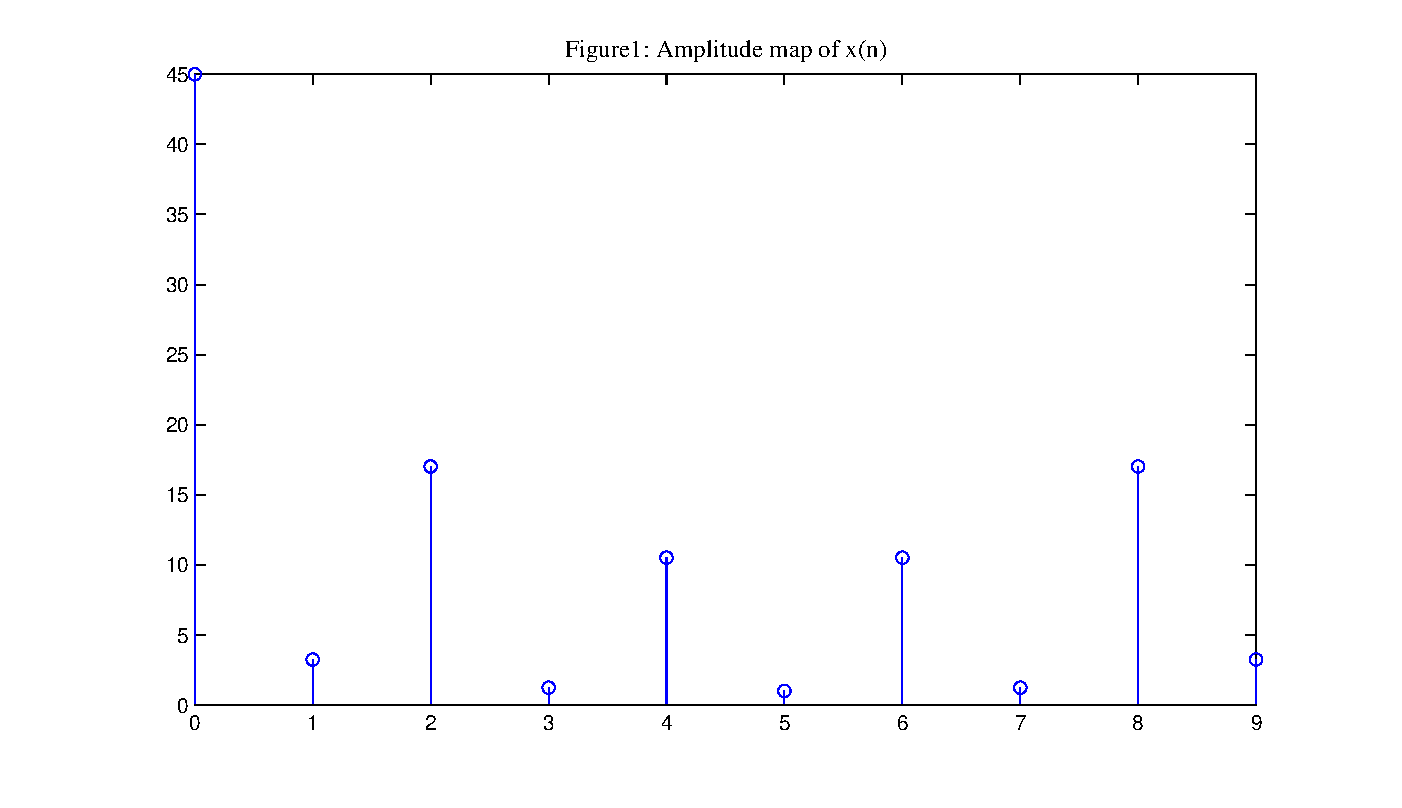
\includegraphics[width=1\textwidth]{fig1.eps}
\end{center}
\begin{center}
    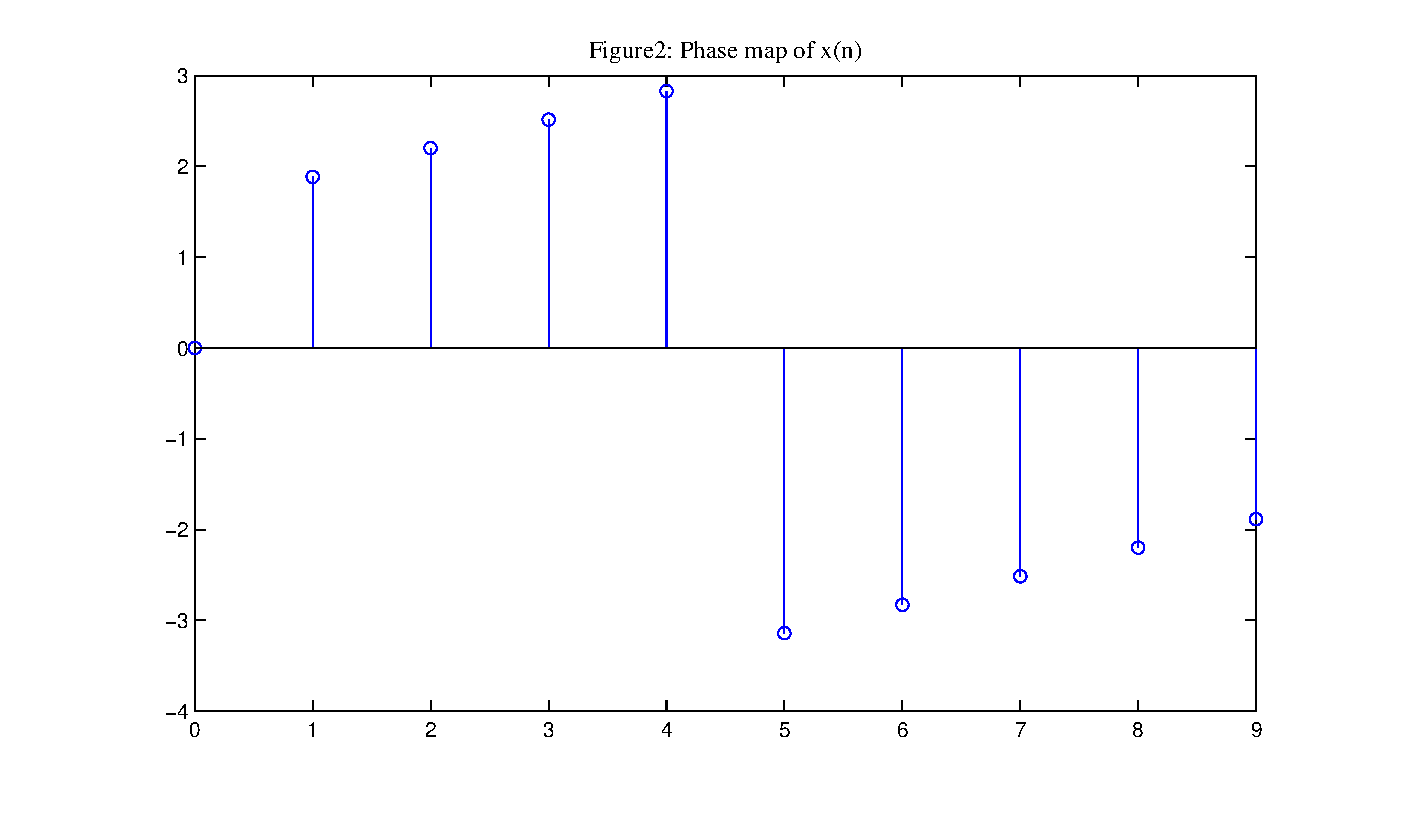
\includegraphics[width=1\textwidth]{fig2.eps}
\end{center}

接下来对另一序列$y(n) = [43, 32, -438, 23.3+87j, -48, 32.47, -10, 0, 12.34+32.56j, 55, 44, 33, 22,$ $11, 66, 77, 34, 32, 45.3, 54.3]$,将$y(n)$和$x(n)$补$10$个$0$后的序列分别进行时域循环卷积和线性卷积,结果如下(此处仅画出其实部进行说明,虚部的思路相同,故未继续画出)

\begin{center}
    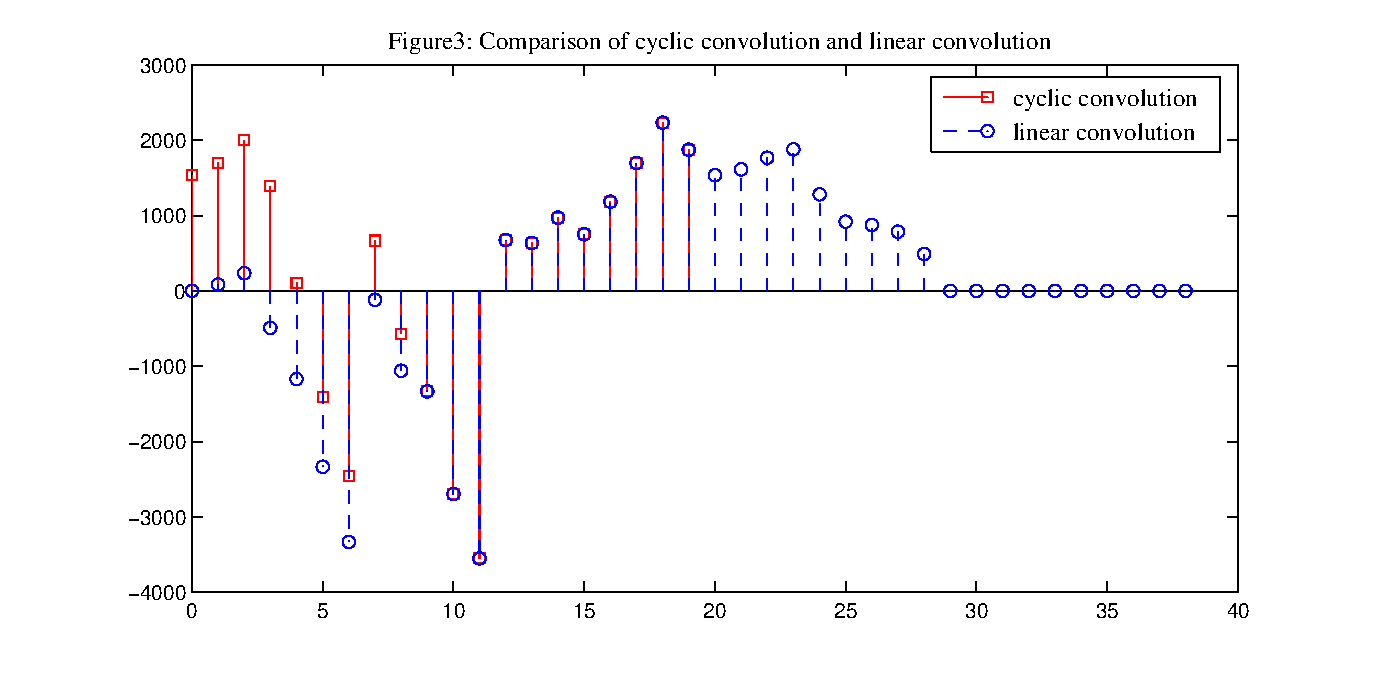
\includegraphics[width=1\textwidth]{fig3.eps}
\end{center}
由图可知,循环卷积长度为$20$个点,线性卷积长度为$39$个点,而取主值序列后为$20$个点,即忽略线性卷积后$19$个点。而从图中我们可以直观的看到循环卷积和线性卷积的前$9$个点取值不同,后面的点取值相同。这是由于发生了混叠造成的,将在后面详细讨论。

接下来对$x(n)$进行补零操作,下图画出原序列、补$10$个零和补$990$个零的$DFT$结果图,包括其幅度谱(左图)以及其相位谱(右图):

\begin{center}
    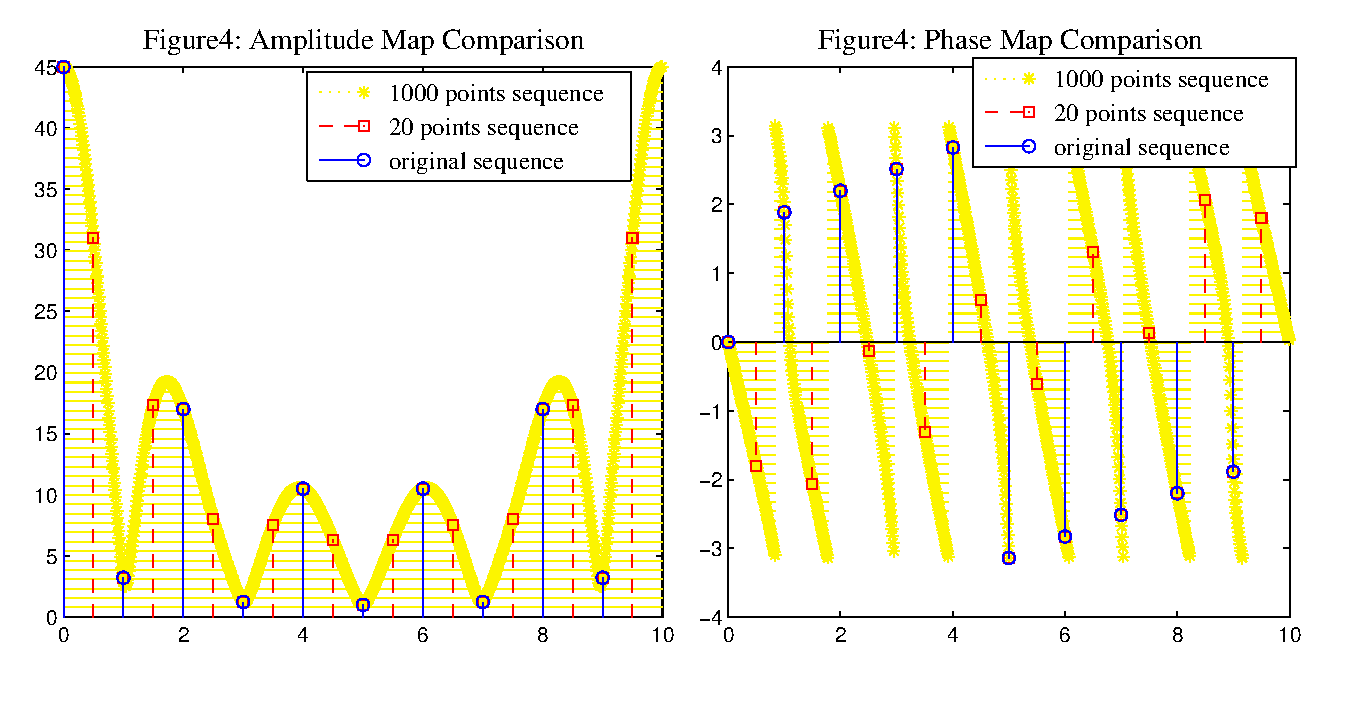
\includegraphics[width=1\textwidth]{fig4.eps}
\end{center}
由图可知补零操作使得频谱变得更密集,克服了所谓的``栅栏效应'',使得频谱的细节捕捉的更清楚。但是注意这只是提高了计算分辨率,而物理分辨率没有改变。之后的讨论也可看到这一点。

求解原序列的$DTFT$如下:

\begin{center}
    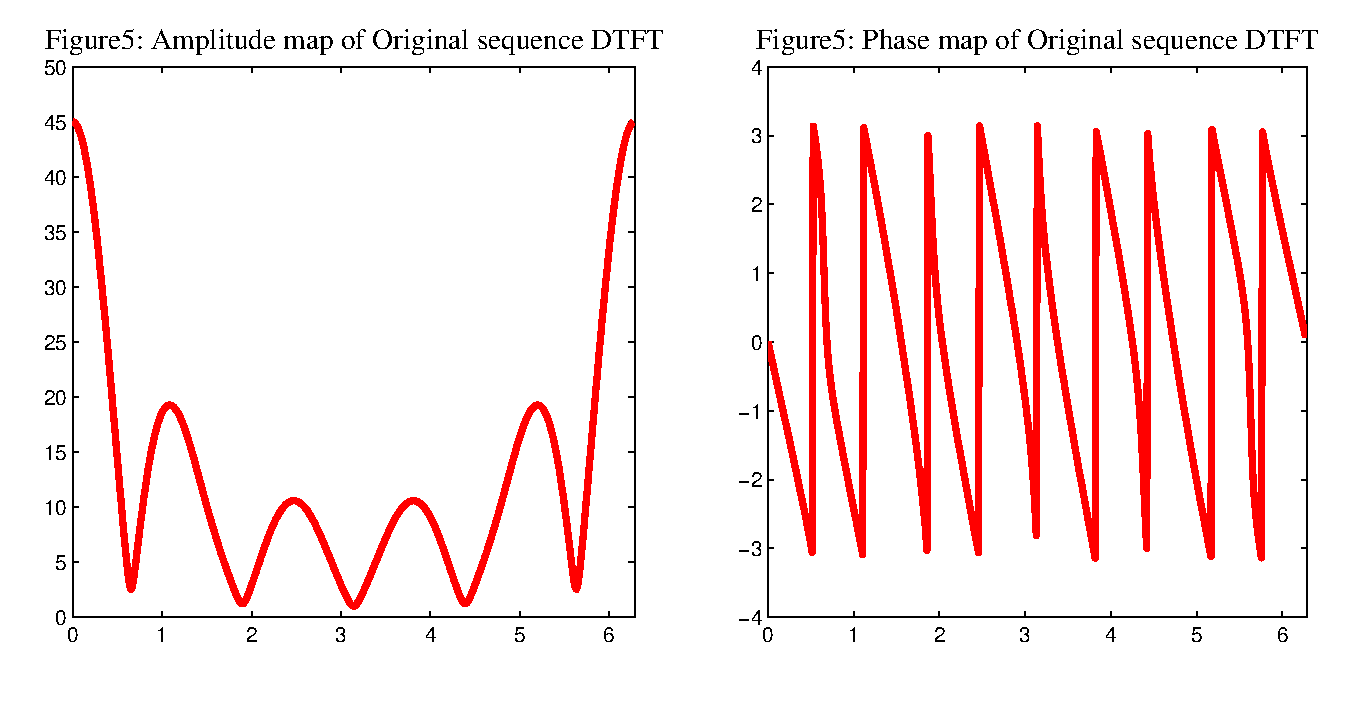
\includegraphics[width=1\textwidth]{fig5.eps}
\end{center}
可见$DFT$只是将$DTFT$进行了离散化抽样,而根据图4可知,点数越多对应能够更清楚的反映原傅里叶变换。

对$x(n)$进行8倍上采样,得到的结果如下,包括其幅度谱(左图)以及其相位谱(右图):
\begin{center}
    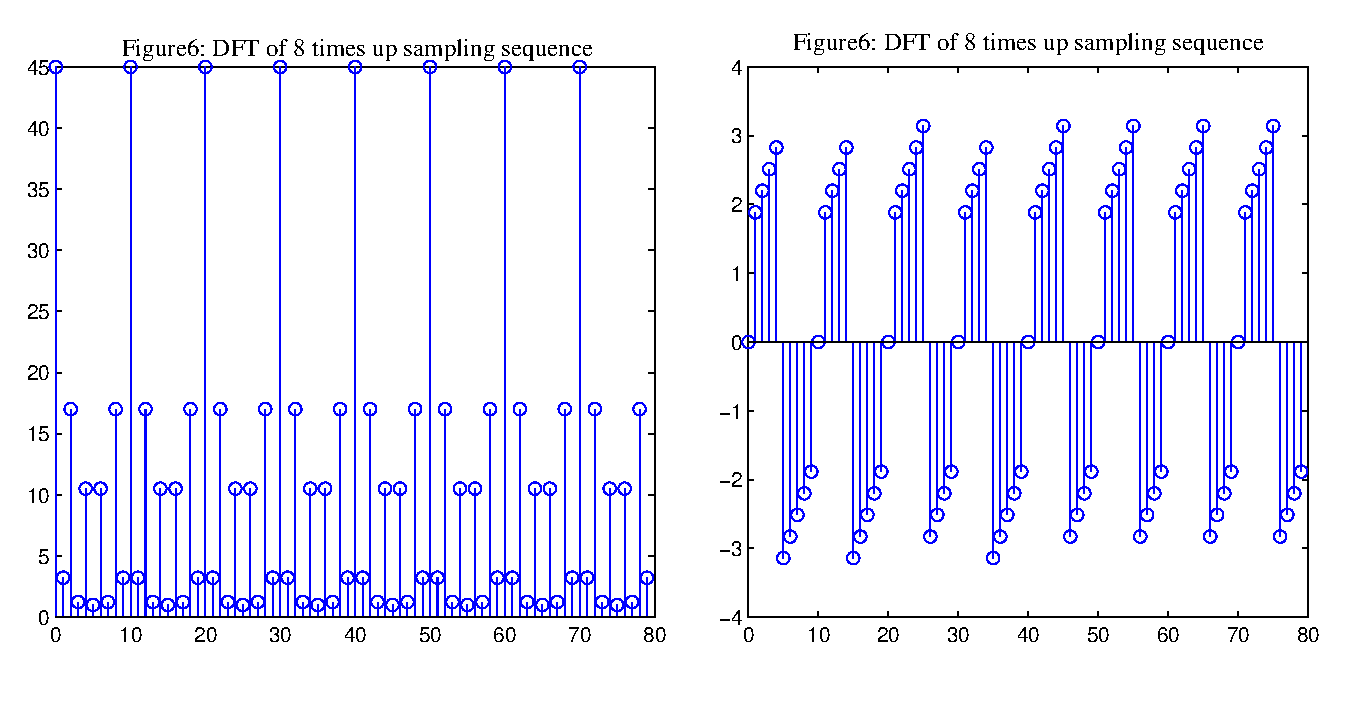
\includegraphics[width=1\textwidth]{fig6.eps}
\end{center}
可见对原序列进行$M$次上采样得到的频谱,对应的是将原序列的离散谱$X(k)$进行$M$次周期循环。证明公式和理由将在后面一节进行详细讨论。

至此,完成了第一题的实验操作。


\subsection{Problem 2}
对于模拟信号$x_a(t)=\sin(2\pi f_0t)+0.5\sin(6\pi f_0t)$,$f_0=1Hz$。选取三种不同的采样频率$f_s$,分别为$5f_0$,$10f_0$和$15f_0$,首先做出采样点图如下:
\begin{center}
    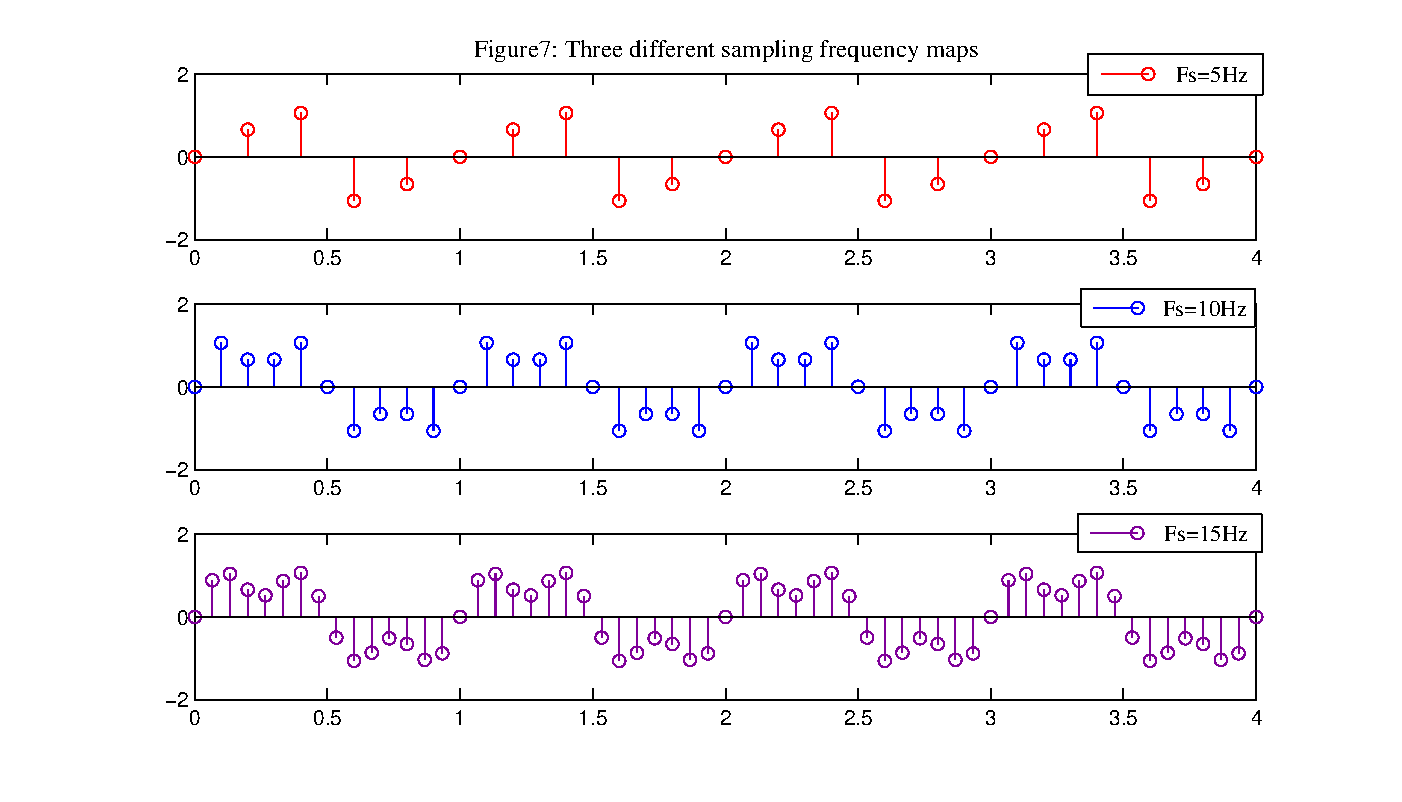
\includegraphics[width=1\textwidth]{fig7.eps}
\end{center}
从图中可以看出$f_s=5f_0$时采样点稀疏,无法反映时域波形特征,而$f_s=10f_0$和$f_s=15f_0$则可以看出时域信号大致波形。对三个采样序列作$FFT$,得到幅度谱分别为(加上了$fftshift$使得零频居中):
\begin{center}
    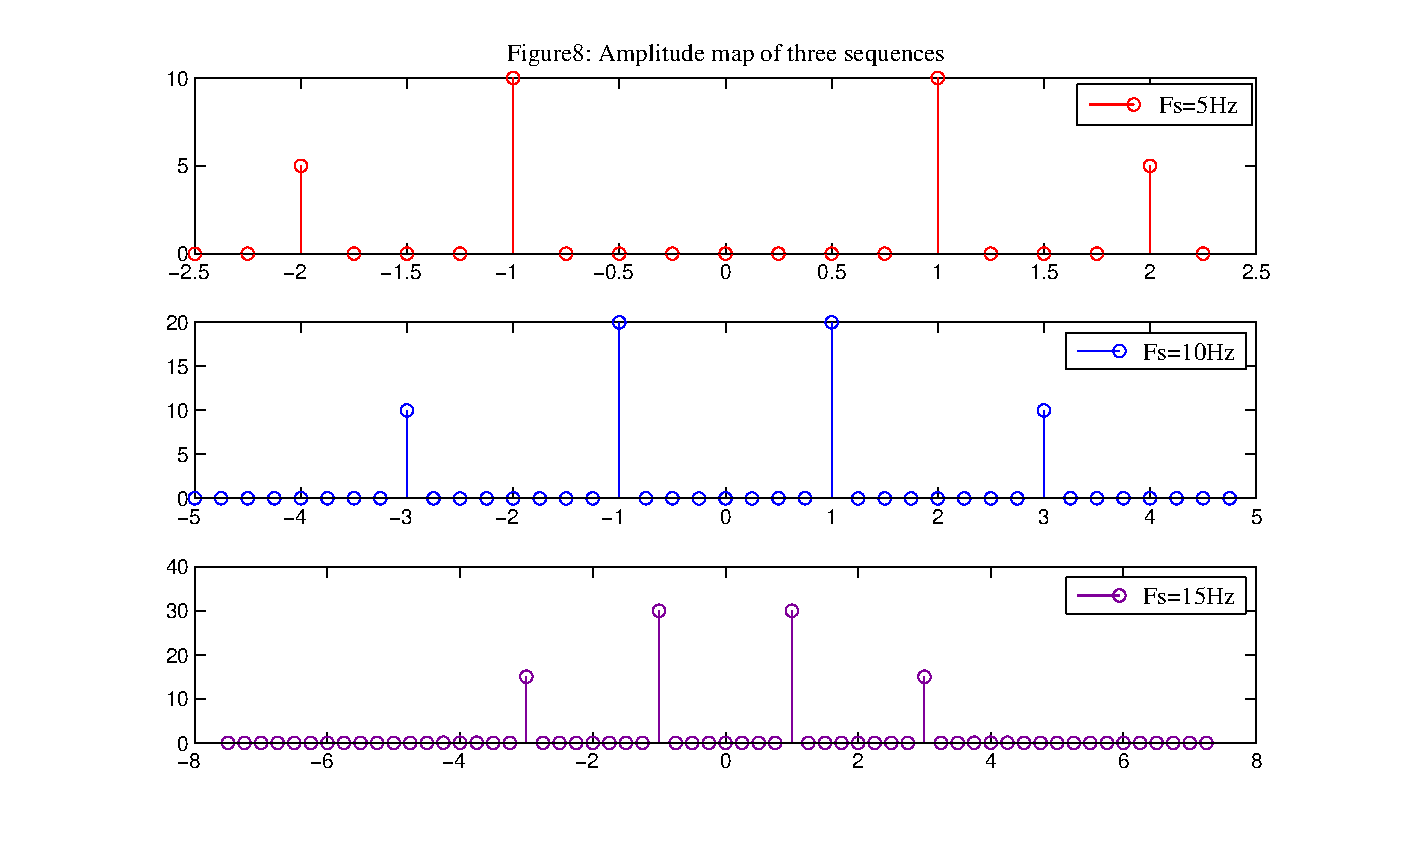
\includegraphics[width=1\textwidth]{fig8.eps}
\end{center}
由此已经可以看出$f_s=5f_0$时频谱发生混叠,看不到$f=3Hz$的频点;而$f_s=10f_0$和$f_s=15f_0$则可以反映原频谱分布。

使用内插公式重建,在此我选择用$f_s=15f_0$重建信号,部分$Matlab$代码如下:

% ===================================插入Matlab代码格式,参考matlab-prettifier文档
\begin{lstlisting}[style=Matlab-editor,
                   basicstyle=\mlttfamily,
                   caption={Reconstruction Code}, label=code1]
N = 30;     %  采样数量
Ts = 1/f3;
n = 0:N-1;    %    时域采样序列
nTs = n*Ts;     %   时域采样时间序列
xs = sin(2*pi*nTs) + 0.5*sin(6*pi*nTs);
t = 0:Ts:1;
%------------------------------内插公式重建
xr = xs * sinc( f3*(ones(length(nTs),1)*t - nTs'*ones(1,length(t))) );
\end{lstlisting}

可以从上述代码第$8$行看到内插公式的使用,在后面的章节会给出原理。结果图如下
\begin{center}
    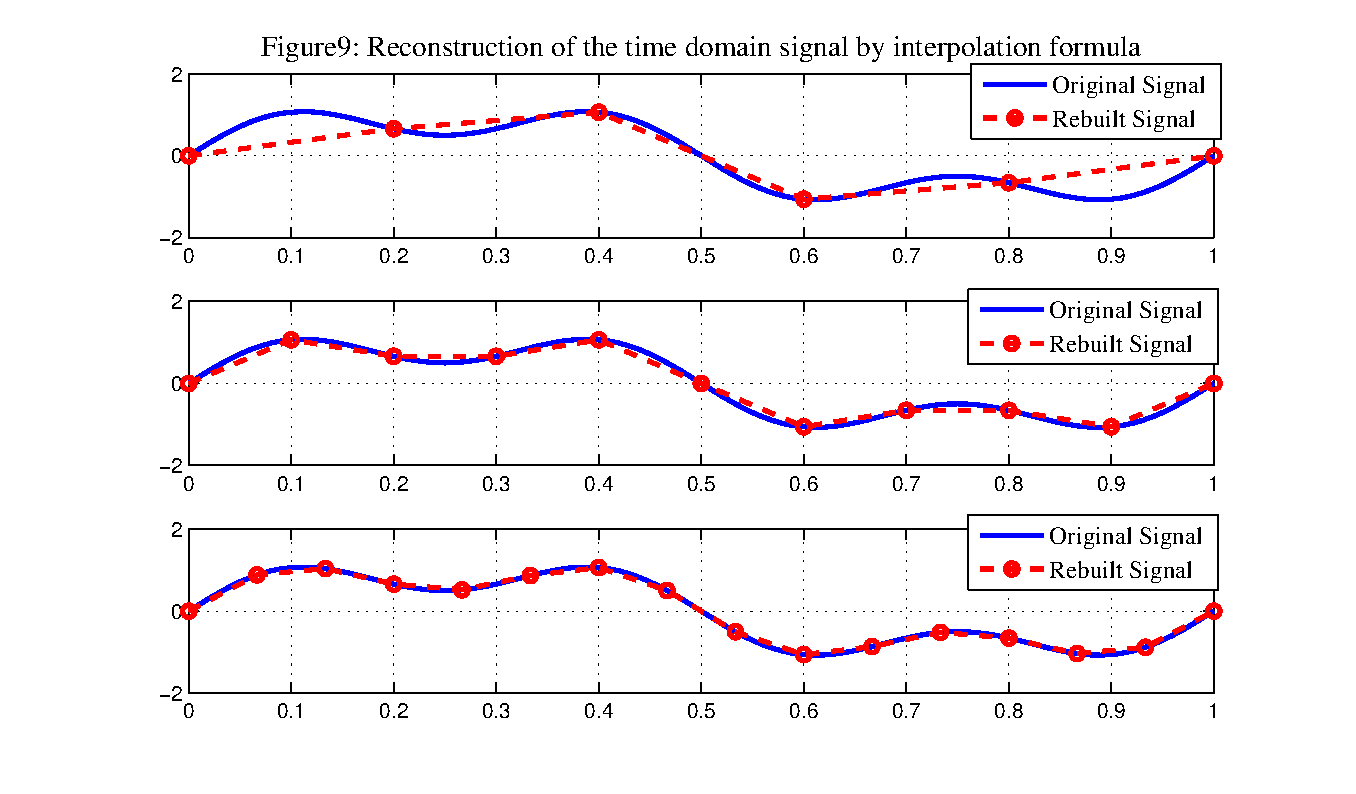
\includegraphics[width=1\textwidth]{fig9.eps}
\end{center}
从图中可以看出,当$f_s=5f_0$时,重建的信号丢失原信号的信息,无法准确恢复原信号;当$f_s=10f_0$时已经可大致重建信号,而当$f_s=15f_0$时重建的信号与原信号几乎一致(之后还需要进行滤波等平滑操作),即可说明时域采样定理。
需要说明的是当采样点越多,恢复的效果就越好。

至此,完成了第二题的实验操作。

\subsection{Problem 3}
如下长度为$M=27$的序列
\begin{equation}
x(n) =
\left\{
\begin{aligned}
& n+1, \qquad 0 \leq n \leq 13. \\
& 27-n, \qquad 14 \leq n \leq 26.
\end{aligned}
\right.
\end{equation}
对其进行$FFT$和$IFFT$,长度$N$分别取$N>M$和$N<M$,在此我取的分别是$N=32$和$N=16(M=27)$。经过频域抽样,变回时域信号后与原信号的对比图,以及频谱对比图如下:
\begin{center}
    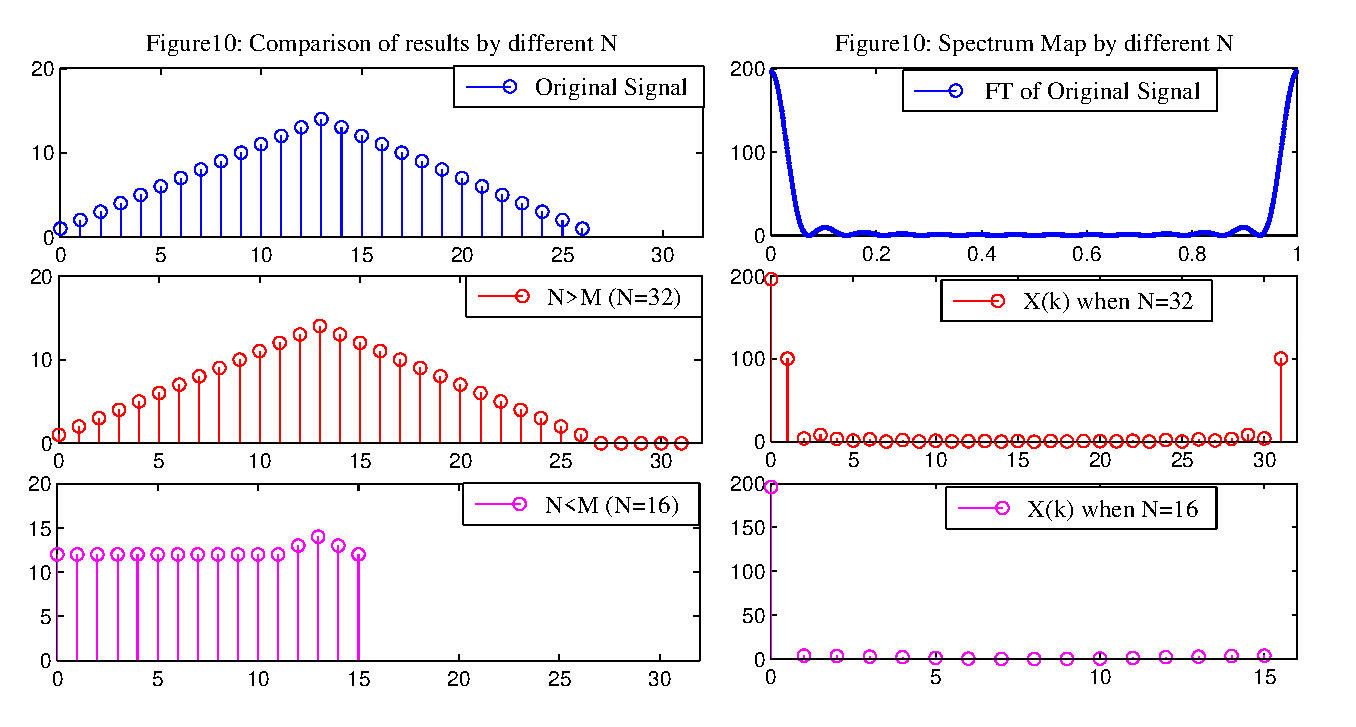
\includegraphics[width=1\textwidth]{fig10.eps}
\end{center}
图中可清楚的看到,当$N>M$时恢复的序列和原序列完全相同;而当$N<M$时则只有前$N$个点有取值,且在前$M-N$个点产生了混叠。这是由于频域抽样本质上是时域信号进行了周期延拓取主值区间导致的。看频谱的情况可以看到,当$N>M$时频谱抽样得到了原频谱的特征,而当$N<M$时则没有,这也验证了频域抽样定理,在后一章节会进行说明。

至此,完成了第三题的实验操作。

\subsection{Problem 4}
对于模拟信号$x_a(t)=\sin(2\pi f_1t)+\sin(2\pi f_2t)+\sin(2\pi f_3t)$,其中$f_1=12Hz$,$f_2=1.25Hz$,$f_3=1.4Hz$,由于$f_2$和$f_3$频率接近,若作$DFT$变换到频域会发生无法分辨的情况,而这又和时域的采样长度有关。

接下来,通过对比不同的时域信号采样长度,以及补零和不补零的区别,来说明物理分辨率和计算分辨率的区别。

首先,对时域信号的数据长度采用$T_0=1s$,而在此试验中抽样频率$f_s=30Hz>2f_{max}=24Hz$,保持$f_s$不变。这样的条件下时域采样点数确定为$N=25$。之后再对此时域序列进行补零至$N^{'}=512$个点,画出对比图如下:
\begin{center}
    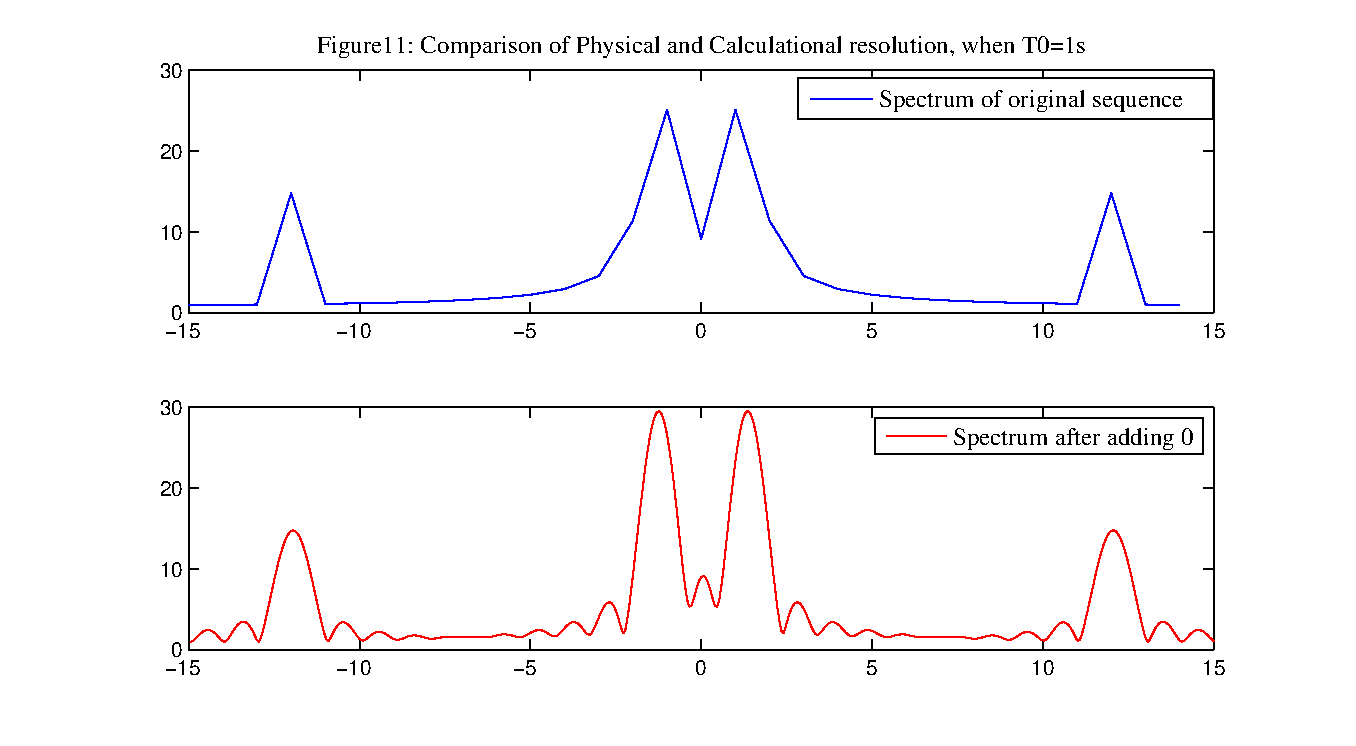
\includegraphics[width=1\textwidth]{fig11.eps}
\end{center}
由图可见,在$T_0=1s$的条件下,原频谱图很粗糙,只能看到在$1Hz$左右和$12Hz$处的两个峰;补零后,频谱图变得细节化,看的更清楚,但是仍然只能看到两个峰。

接下来改变时域数据长度为$T_0=5s$,此时采样点数变更为$N=125$。之后仍然对比不补零和补零至$N^{'}=512$个点,画出对比图如下:
\begin{center}
    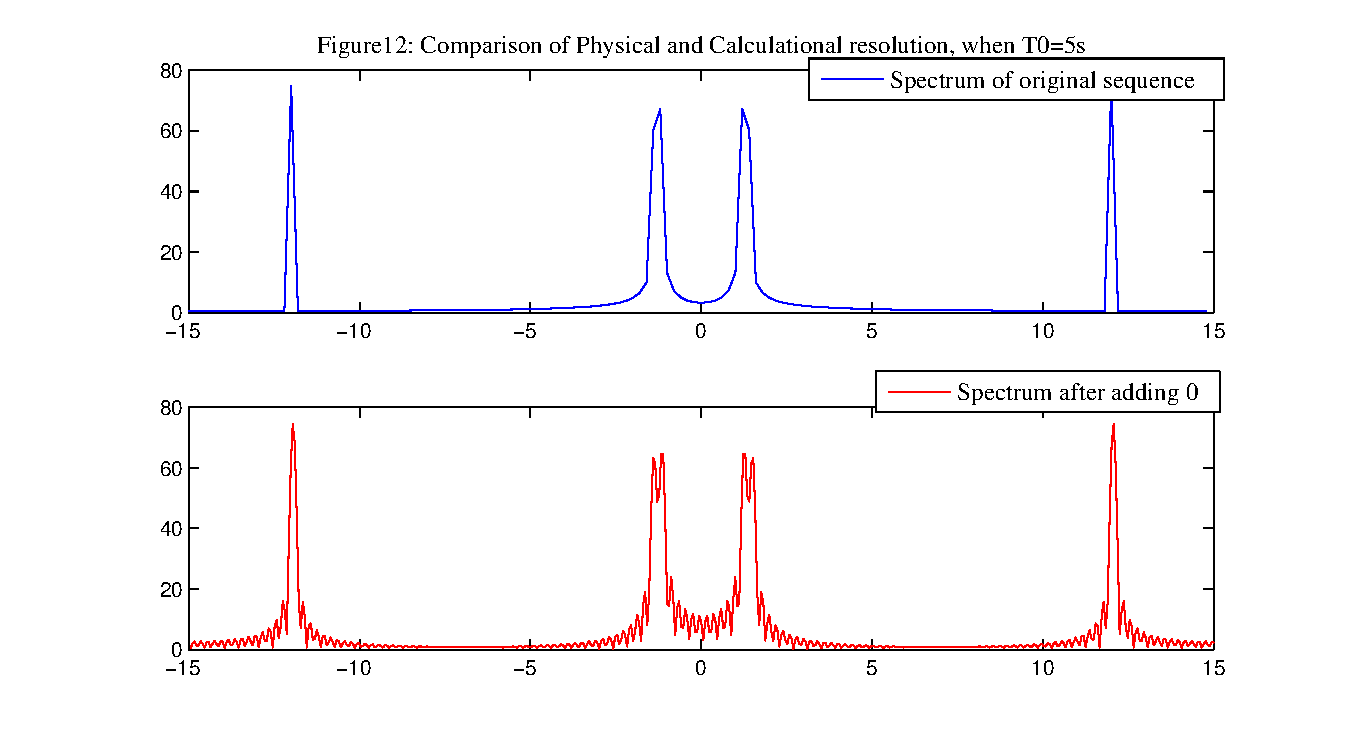
\includegraphics[width=1\textwidth]{fig12.eps}
\end{center}
由图可见,在$T_0=5s$的条件下,原频谱图细节更好了,虽然仍然只能看到在$1Hz$左右和$12Hz$处的两个峰;而在补零后,我们可以清楚地看到在$1Hz$左右的峰分化为两个,成功的看到了$f_2=1.25Hz$和$f_3=1.4Hz$两个频点。

关于本题的说明(频谱泄漏问题等)在下一节进行详细讨论。至此,完成了所有实验操作和数据处理。

\section{实验结果分析}

\subsection{Problem 1}

\subsubsection{Problem 1.1}
相位谱和幅度谱分别在图$1$和图$2$中给出,其中看相位谱会发现在第$5$点和第$6$点间会有一个相位的突变,这可以根据原序列通过$DFT$变换后的表达式得出,并且通过图可以看出相位谱是在$[-\pi,\pi]$间取值。

\subsubsection{Problem 1.2}
循环卷积和线性卷积的联系是:$N$点圆周卷积$y(n)$是线性卷积$y_l(n)$以$N$为周期的周期延拓序列的主值序列~\supercite{course2}。而要想满足循环卷积等于线性卷积的条件,则是:
\begin{equation}
N \geq N_1+N_2-1, \quad s.t. \ \ y(n) = y_l(n).
\end{equation}
其中$N$为循环卷积的长度,$N_1$、$N_2$分别为两序列长度。

本问中由于$N_1+N_2-1=39>20=N$,故会发生混叠;而由于$x(n)$是在后面补了$10$个零,故有效序列长度仍为$10$,即有循环卷积的前$9$个点会发生混叠,从图中也可以直观看出,线性卷积的$(20\sim 28)$点分别加在$(0\sim 8)$点上,就是相应的循环卷积的值(代码$pro1\_2.m$ 中有相关语句,加上后运行可发现两卷积的主值序列完全相同,验证了其正确性)。

\subsubsection{Problem 1.3}
本问比较了在序列$x(n)$的末尾补零对其$DFT$的频谱图影响问题,可以看到补零有效的解决了``栅栏问题'',使得原本稀疏的频谱~(蓝点显示 的)变得密集许多,细节可以看的更加清楚,通过对比图$4$和图$5$即可看出。但是需要注意的是补零并没有改变频谱,也即只是提高了计算上的分辨率,在原来的谱线之间进行了线性插值;而原本谱线所不能反映的~(e.g., 两个距离很近的频谱峰),补零后仍然不能反映。

\subsubsection{Problem 1.4}
由图6可以看到,进行8倍上采样实际上是把原$DFT$频谱进行了循环延拓8次。记进行8倍上采样的序列为$x^{'}(n)$,原序列为$x(n)$,具体证明如下:
\begin{equation}
\begin{split}
X^{'}(k) = & \sum_{i=0}^{rN-1} x^{'}(i)W_{N}^{ik}R_{N}(rN-1) \\
= & \sum_{i=0}^{rN-1}x(\frac{i}{r})W_{N}^{\frac{i}{r}k} R_{N}(rN-1) \\
= & \sum_{m=0}^{N-1} x(m)W_{N}^{mk}R_{N}(rN-1), \qquad m = 0,1,\cdots,N-1.
\end{split}
\end{equation}
其中$r$为上采样倍数。由于$X^{'}(k)$为$rN-1$点序列,当$k>N-1$时,其取值与对应$[0,N-1]$上的取值一样,故本质上进行进行8倍上采样,实际上是把原$DFT$频谱进行了周期循环延拓8次。

\subsection{Problem 2}

\subsubsection{Problem 2.1}
采样点图见图7,从图中可以看出$f_s=5f_0$时采样点稀疏,无法反映时域波形特征,而$f_s=10f_0$和$f_s=15f_0$则可以看出时域信号大致波形。这也从时域的角度说明了时域采样定理,当采样频率过低时,采样序列是无法准确反映出其特征的。

\subsubsection{Problem 2.2}
做了$FFT$后,由图8可以看出$f_s=5f_0$时频谱发生混叠,看不到$f=3Hz$的频点;而$f_s=10f_0$和$f_s=15f_0$则可以反映原频谱分布。这是由于$f_s=5f_0$时不满足时域抽样定理$f_s \geq 2f_h$,导致结果的频谱最高值为$f_s$的一半$2.5Hz$,故无法看到$f=3Hz$的频点。
由此可以验证时域采样定理。

\subsubsection{Problem 2.3}
由满足采样定理的抽样序列,通过插值公式:
\begin{equation}
x_a(t) =  \sum_{n = -\infty}^{\infty} x(nT_s) \frac{\sin[\pi (t-nT_s) / T_s]}{\pi (t-nT_s) / T_s}.
\end{equation}
即可重建原信号。由图9也可以看出,$f_s=15f_0$时重建信号与原信号几乎一致(通常还要通过低通滤波等后续处理)。由于时域抽样间隔为$T_s$,若增大抽样点,即减小$T_s$,可以获得更加精确的重建信号。

\subsection{Problem 3}
频域抽样定理告诉我们~\supercite{course1,course2},若原序列$x(n)$的长度为$M$,则只有当频域抽样点数$N\geq M$时,才有$x_{N}(n) = IDFT[X(k)] = x(n)$,即可由频域抽样$X(k)$恢复原序列$x(n)$。这说明$x_N(n)$为原序列$x(n)$以$N$为周期的周期延拓序列的主值序列,也即
\begin{equation}
x_N(n) = \tilde{x}_N(n)R_N(n) = \sum_{r = -\infty}^{\infty}x(n+rN) R_N(n).
\end{equation}

在此问题中,当$N>M$ 时恢复的序列则和原序列完全相同;而当$N<M$时,由图10可以看到只有前$N$个点被恢复,且前$M-N$个点发生了混叠,这是由于周期延拓所导致的,因延拓的周期$N$ 比原序列长度$M$要小,故在延拓前要将后$M-N$个点先加到前面,即发生了混叠。这由频谱图也可直观看出,当$N<M$时频域抽样值不足以恢复原频谱。
由此,频域抽样定理得以验证。

\subsection{Problem 4}
图12给出物理分辨率和计算分辨率的区别实验结果,在$T_0=1s$的条件下,原频谱图很粗糙,只能看到在$1Hz$左右和$12Hz$处的两个峰;补零后,频谱图变得细节化,看的更清楚,但是仍然只能看到两个峰。而在$T_0=5s$的条件下,原频谱图细节更好了,虽然仍然只能看到在$1Hz$左右和$12Hz$处的两个峰;而在补零后,我们可以清楚地看到在$1Hz$左右的峰分化为两个,成功的看到了$f_2=1.25Hz$和$f_3=1.4Hz$两个频点。

物理分辨率定义为
\begin{equation}
F = \frac{1}{T_0}.
\end{equation}
$T_0=5s$的条件实际等效为加长了原序列数据的长度,这样可以减小频率的物理分辨率,从而增加了精度。而当$T_0=1s$时可以看出无论如何补零都无法分辨接近的两个频率,这也说明了当数据长度小,对应的物理分辨率就大,精度就低。补零是无法改变物理分辨率的,这也从实验结果可以看出,就不再赘述。而其本质原因是:补零导致的中间加上的部分只是对$DFT$结果插值作用,克服栅栏效应使得稀疏的序列变得光滑而已,而频率分辨率还是只是原有的谱线间隔。补零的实际效果相当于增加了计算分辨率,看的东西更多了而已。

这里通过结果,又引出了另一个问题:频谱泄漏问题。本题中仅有三个频率点,但是在结果中却看出频谱发生了延拓,实则为频谱泄漏现象。这是由于取样的时间序列长度不是其周期的整数倍造成的。分析如下:

由于为周期无限长序列,我们只取其一部分,而在做$FFT$变换时会将这个截断后的信号进行重构,倘若信号截断的长度不为原始信号周期的整数倍,则在连接处信号的幅值不连续,会出现跳跃的情况,进而导致频谱较原来发生改变。在图11、12中可以看到,频谱在整个频带上发生``拖尾''现象。峰值处的频率与原始信号的频率相近,但并不相等。从数学上分析如下:

对单频信号的周期截断而言,假设原始信号的频率为$f$,则周期为$1/f$。因为截取的时间长度$T$为信号周期的整数倍(假设为$k$倍),即
\begin{equation*}
T = \frac{k}{f}.
\end{equation*}
而频率分辨率为$1/T$,即
\begin{equation*}
F = \frac{1}{T} = \frac{f}{k}.
\end{equation*}
因而,信号的频率成分
\begin{equation*}
f = k \cdot F.
\end{equation*}
即信号的频率成分为频率分辨率$F$的整数倍,也就是说频谱图中有一条谱线与信号的频率成分相同,这也就是所谓的信号``压谱线''。而当非周期截断时,由于非周期截断的时间长度不等于信号周期的整数倍,因此信号的频率成分$f \neq k \cdot F$,也就是说在频谱图中,没有一条谱线与信号的频率成分完全相同。

由于本题中的信号的周期为$T_s=20s$,故再次取数据长度$T_0=20s$,得到下图:
\begin{center}
    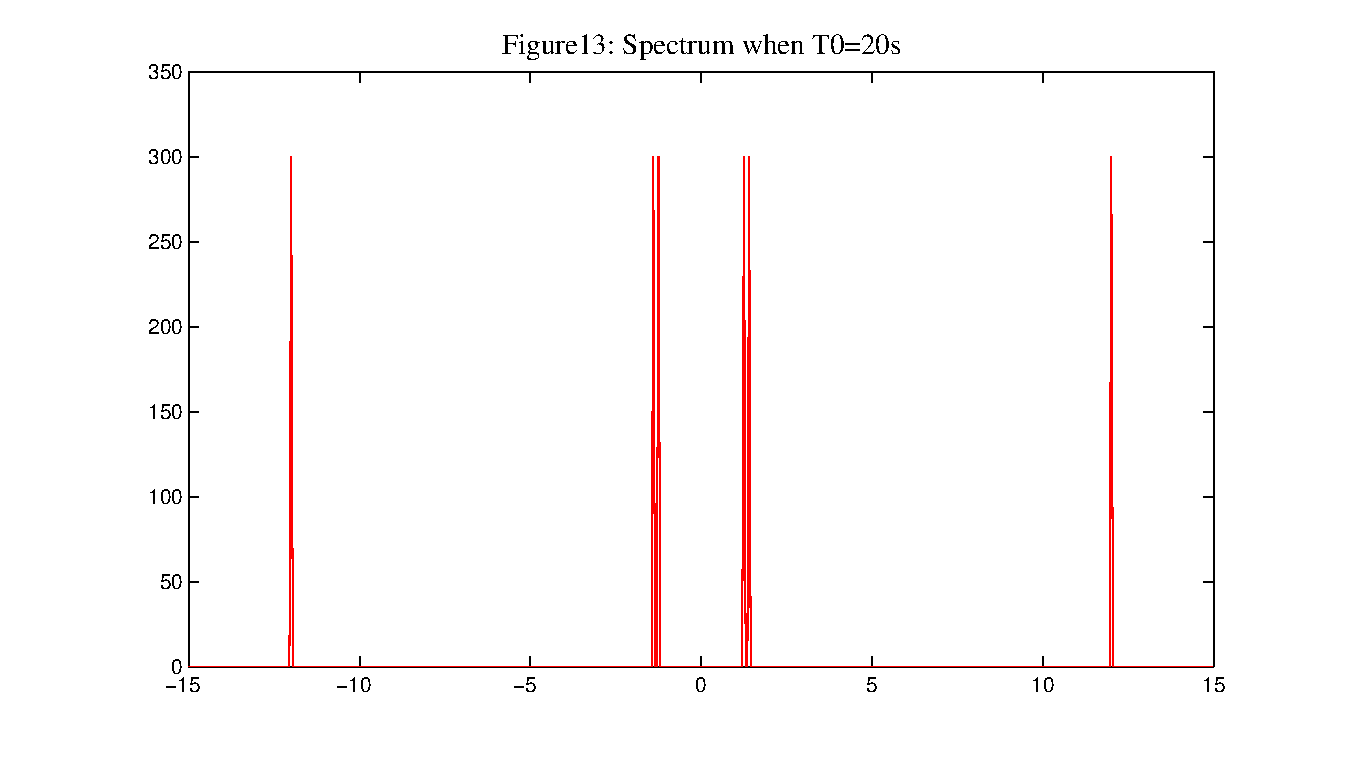
\includegraphics[width=1\textwidth]{fig13.eps}
\end{center}
从图中可清楚的看到只有三根谱线,分别对应原$f_1,f_2,f_3$的取值。而取$T_0=20s$也再次说明了物理分辨率是由数据长度决定的,数据长度越长其分辨率的精度越高,而补零只能增加计算分辨率。

\section{总结}

本次报告对关于$DFT$、$FFT$和抽样等内容做了介绍,完整完成了实验过程并给出了数据图,最后作出了详细的结果分析。经过本次实验,本人对离散傅里叶变换有了更深的理解,并对较晦涩难懂的内容,例如物理/计算分辨率,梳理得更加清楚。本次实验也让我认识到了自己的不足之处,对给出的问题需要思考较久思路,说明对课堂内容没有完全吃透,之后还要多加注意。


\section{附录}
$Matlab$代码名称对应问题的题号~(和相应小问),使用是添至搜索路径运行即可,注意某些函数中用到了自己写的$DFT/IDFT$函数。

由于要画的图中部分序列存在虚部,而实部和虚部所对应的结果说明的问题一样,但是不能简单的取模(例如线性和循环卷积,若只是取模则看不到叠加后两个序列相同的结果),故部分图只画出其实部。

本文的图片均为$.eps$格式,可以进行缩放而不失真的矢量图,在观察某些细节(例如物理分辨率那张图)时观察得更清楚。由于$Matlab$含有中文的图片在导出$.eps$文件时会出现乱码情况,故所有图片的标题等均为英文所写。

最后,由于报告中需要加入许多数学表达式,本文档使用了$LaTeX$来编写报告,以获得更优的排版效果。
\iffalse
\footnote{Here you can add some footnotes.}。
\fi


% =====================================================Reference
\small
\begin{thebibliography}{99}
\setlength{\parskip}{0pt}  %段落之间的竖直距离

\bibitem{wiki}
https://zh.wikipedia.org/wiki.

\bibitem{textbook}
程佩青. 数字信号处理教程~(第三版), 清华大学出版社, 2012.6.

\bibitem{wikifft}
Brenner, N.; Rader, C. A New Principle for Fast Fourier Transformation. \emph{IEEE Acoustics, Speech \& Signal Processing}. 1976, 24(3): 264–266.

\bibitem{course1}
尚勇. 离散傅里叶变换, 第三讲. 2017, 3.

\bibitem{course2}
尚勇. 离散傅里叶变换, 第四讲. 2017, 3.

\bibitem{course3}
尚勇. 快速傅里叶变换. 2017, 3.

\end{thebibliography}

\clearpage
\end{document}
